\documentclass{article}
\usepackage[a4paper,top=2cm,bottom=2cm,left=2cm,right=2cm]{geometry}
\usepackage[english]{babel}
\usepackage[T1]{fontenc}
\usepackage[utf8]{inputenc}
\usepackage{fancyhdr}
\usepackage{float}
\usepackage{graphicx}
\usepackage{wrapfig}
\usepackage{siunitx} %per scrivere il simbolo °
\usepackage{verbatim} %per i commenti1
\usepackage{amsmath}
\usepackage[linesnumbered, ruled, vlined]{algorithm2e}
\setcounter{secnumdepth}{3}
\setcounter{tocdepth}{6}
\usepackage{multirow}
\newcommand{\minitab}[2][l]{\begin{tabular}#1 #2\end{tabular}}
\usepackage{rotating}
\usepackage{xfrac}
\usepackage{cite}
\usepackage{caption}
\usepackage{subcaption}
\usepackage{hyperref}

\DeclareMathOperator*{\argmax}{arg\,max}
\DeclareMathOperator*{\argmin}{arg\,min}

%\usepackage{booktabs,array}
%\usepackage{tikz}

%\usepackage{tabularx}

%\usepackage{chngcntr}
%\counterwithin{table}{section}

%------------------------------ colors
\usepackage[usenames,dvipsnames,table]{xcolor} % use colors on table and more
\definecolor{333}{RGB}{51, 51, 51} % define custom color
\definecolor{background}{RGB}{248, 248, 255}
\definecolor{comment}{RGB}{17,167,5}
\definecolor{keyword}{RGB}{195,47,8}
\definecolor{string}{RGB}{142,195,0}
\definecolor{number}{RGB}{90,84,84}
\definecolor{identifier}{RGB}{0,90,201}

%------------------------------ source code
\usepackage{listings}

\lstset{
  basicstyle=\footnotesize\sffamily,
  commentstyle=\itshape\color{gray},
  captionpos=b,
  frame=shadowbox,
  language=HTML,
  rulesepcolor=\color{333},
  tabsize=2
}

\usepackage{xcolor}
\hypersetup{
    colorlinks,
    linkcolor={blue!50!black},
    citecolor={blue!50!black},
    urlcolor={blue!80!black}
}

\title{\textbf{Report about Project}} % Title
\author{Raffaele \textsc{Di Nardo Di Maio} 1204879} % Author name
\date{\today}

\begin{document}
\begin{minipage}{.20\textwidth}
  
\includegraphics[height=3cm]{../Icon4}
\end{minipage}\begin{minipage}{.20\textwidth}
  \begin{table}[H]
  \begin{tabular}{l}
  \scshape{\Large{Computer Engineering Master Degree}} \\
  \hline \\
  \scshape{\Large{Computer Vision}} \\
  \end{tabular}
  \end{table}
\end{minipage}
{\let\newpage\relax\maketitle}

\section{Method used}
\subsection{Project details}\label{details}
The goal of the experience was to find in an image the best match from a set of views of an object that we are trying to localize. The steps followed by the implemented program, to reach the goal, are the following:
\begin{enumerate}
\item{\textbf{Computation of $\gamma$-transform}\\
the used gamma values are all greater than 1. This transform is applied to increase the contrast and stretch very high pixel values in an image. This operation is performed only on views because of their very high brightness.}
\item{\textbf{Computation of Canny detection}\\
Canny detector is applied to the test images and also to the $\gamma$-transformed views.}
\item{\textbf{Matching phase}\\
this phase is performed using two different approaches, depending on the specification of the optional argument \texttt{-dist} (see Section \ref{args}). These approaches are:
\begin{itemize}
\item{\textbf{Template Matching with distance transform}\\
The distance transform is applied to each test image with detected edges. Then the function \texttt{cv::matchTemplate()} is applied to the result of the transform using, as templates, the views on which Canny was applied. The metric used is the \textit{Correlation Coefficient (TM\_CCOEF} in opencv\textit{)}. Then the max value of an element in the resulting matrix is kept and its position is used as the location of the template for the corresponding match. With this approach I take only the ten best matches for each image, as specified in the assignment, by looking only at the best matches of each view in that image. The score value used to establish the best matches is the value contained in the max entry of the result matrix.
}
\item{\textbf{Template Matching with histogram refinement}\\
Template matching is performed on the test image (on which Canny was applied) and using view images processed with Canny as templates, looking at TM\_CCOEF as in the previous approach. To improve the results obtained, I don't take only the 10 best matches for a test image but the 50 best results and then I apply a histogram-based refinement algorithm. For each one of the 50 matches I take a sub-window, related to the position of the match and with size equal to the related view, and I filter it with the corresponding mask. This RGB sub-window of the original test image is then converted to the HSV space and the histogram of its Hue channel is computed. The resulting histogram is then compared with the Hue histogram of the original view image using \texttt{cv::compareHist()}. The final score assigned to a match is the composition of the sliding window score and the histogram comparison score:
$$final\_score=\alpha*match\_score + \beta*hist\_score$$
where \textit{match\_score} is the score obtained by applying only \texttt{cv::matchTemplate()} and \textit{hist\_score} is the score obtained through \texttt{cv::compareHist()}. Hence from the initial set of 50 best matches obtained through template matching, based on sliding window, I only take the 10 best matches w.r.t. new final score.}
\end{itemize}
}
\item{\textbf{Generation of result text files and result images}\\
for each of the 10 best matches, the edges of its mask are highlighted in red and printed on the position evaluated before over the image. Each result image has a name with this format:
\begin{center}
\begin{tabular}{c}
\begin{lstlisting}[linewidth=120pt, basicstyle=\footnotesize\sffamily,]
datasetNum_matchNum.jpg
\end{lstlisting}
\end{tabular}
\end{center}
where \texttt{datasetNum} is the name of the dataset folder (it can be \textit{can}, \textit{driller} or \textit{duck}) followed by the number of the corresponding test image and \texttt{matchNum} is an integer number in $[0,9]$ that identifies the quality of the score of a match in the set of 10 best matches (\texttt{0} for higher score, \texttt{9} for lower score).\\
The edges of the view that matches in the test image are highlighted in red. For each dataset the matches are written in the corresponding results text file with the format specified in the assignment.}
\end{enumerate}

\subsection{Experimental results}\label{exp}
Looking at the details of the previously analysed steps of the implementation, I explain the reasons and the results obtained with the previous operations:
\begin{enumerate}
\item{\textbf{Computation of $\gamma$-transform}\\
The $\gamma$-transform was applied after different trials because of the presence of too many weak edges and because of the colours of the views. Instead of using this transform, I tried to equalize the images but the results were worse than those obtained without any single-pixel operations. After several trials, the final values of $\gamma$ in $\gamma$-transform applied to each set of views are the following:
\begin{table}[H]
\footnotesize\centering
\begin{tabular}{rccc}
\cline{2-4}
& \textbf{can} & \textbf{driller} & \textbf{duck}\\
\hline
{$\mathtt{\gamma}$} & {1.4} & {1.3} & {1.4}\\
\hline
\end{tabular}
\caption{$\gamma$ values for $\gamma$-transform applied on views of each dataset.}
\end{table}
}
\item{\textbf{Computation of Canny detection}\\
For each dataset I defined two different high thresholds of the Canny detector for each dataset: the first for the views and the second for the test images. Then, looking at the results obtained, I assigned to the low thresholds of Canny detector the values of the high thresholds decreased by a specific quantity: 30 for views and 40 for the test images. The values for high thresholds are the following:
\begin{table}[H]
\footnotesize\centering
\begin{tabular}{rccc}
\cline{2-4}
& \textbf{can} & \textbf{driller} & \textbf{duck}\\
\hline
\textbf{test images} & {150.0} & {150.0} & {100.0}\\
\hline
\textbf{views} & {100.0} & {160.0} & {100.0}\\
\hline
\end{tabular}
\caption{High thresholds for the Canny detector.}
\end{table}
The high thresholds of the \textit{duck} dataset are both smaller than the others  because more details are needed to correctly detect the shape of the wing and the beak of the object.
}
\item{\textbf{Matching phase}\\
In this phase for each image of each dataset, the two methods obtain both all the best feasible matches. In several cases the correct match isn't the match with highest score (e.g. Figure \ref{example_matching}). For both approaches, the matching was more simple on the \texttt{can} dataset and very complex for images of the \texttt{driller} and \texttt{duck} datasets.\\
The main problem of these methods based on histogram refinement was to find the best thresholds for Canny detection of \texttt{driller} and \texttt{duck} because of many problems based on their shapes. In particular for \texttt{driller} matching, too small values for the high Canny threshold help me to identify better the object in some images but increase the loss of correct matches on other ones. The same happens with too big values for the high Canny threshold. The reason comes from the level of contrast of different images and the smoothness of some of them.\\
In particular, the method with the distance transform is more efficient in terms of memory occupation because it stores less results.
As explained before, the histogram comparison performed during the Refinement phase only involved the Hue channel of the HSV colour space. I did not work with the RGB colour space because the test image objects and their corresponding models differed in luminosity and saturation. I tried another approach to estimate the final score from the histogram comparison without combining it with the previous one. I tried to use only the histogram comparison score to discover, from the set of 50 best matches, the new 10 best ones. The two approaches implemented were: 
\begin{itemize}
\item{take only matches with the histogram comparison score greater than a specified threshold;}
\item{take the 10 matches with the highest histogram comparison score}
\end{itemize}
For both methods, I noticed that having higher histogram comparison scores doesn't mean that there will not be false positives. For this reason I decided to give a higher weight to the previous Template Matching score and combine it with the histogram comparison score in the following way:
$$final\_score=100*match\_score + hist\_score$$
The coefficients were computed after trying several combinations of them.}
\end{enumerate}
\begin{figure}[H]
\begin{subfigure}{.5\textwidth}
  \centering
  % include third image
  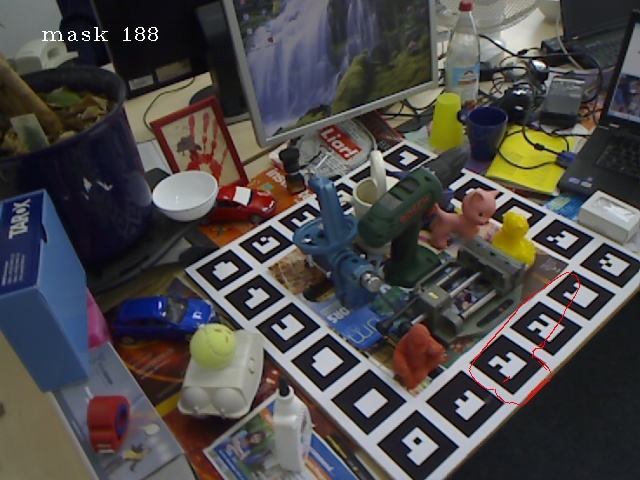
\includegraphics[width=.9\linewidth]{Images/driller_score1.jpg}  
  \caption{Match with the highest score on test1.jpg.}
\end{subfigure}
\begin{subfigure}{.5\textwidth}
  \centering
  % include fourth image
  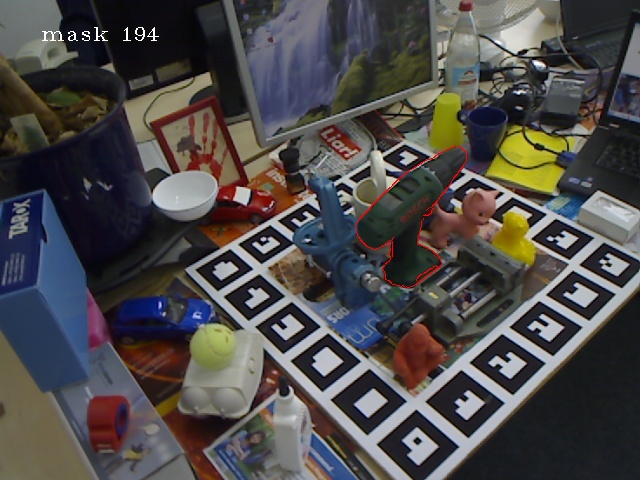
\includegraphics[width=.9\linewidth]{Images/driller_best1.jpg}  
  \caption{Correct match on test1.jpg.}
\end{subfigure}
\newline
\vspace{0.5cm}
\begin{subfigure}{.5\textwidth}
  \centering
  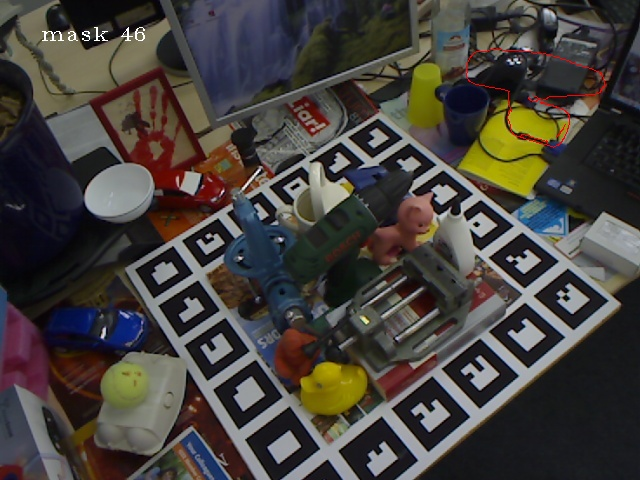
\includegraphics[width=.9\linewidth]{Images/driller_score3.jpg}  
  \caption{Match with the highest score on test3.jpg.}
\end{subfigure}
\begin{subfigure}{.5\textwidth}
  \centering
  % include fourth image
  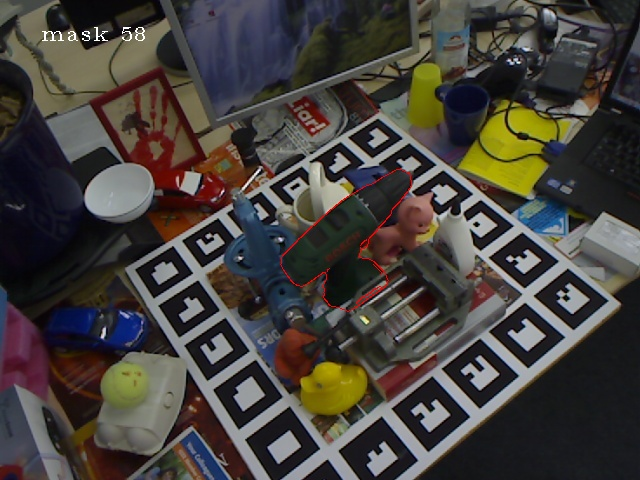
\includegraphics[width=.9\linewidth]{Images/driller_best3.jpg}  
  \caption{Correct match on test3.jpg.}
\end{subfigure}
\caption{Comparison between the highest score match and the correct match on two images of the \texttt{driller} dataset.}
\label{example_matching}
\end{figure}

\section{Code}
\subsection{Performance}
The program can analyse only one dataset or all the datasets in parallel. The management of this behaviour was done using threads. Each thread performs the template matching on a dataset and the terminal window, for log printing, is the only resource managed using mutual exclusion.\\
Referencing to Section \ref{details}, I'm going to discuss the little tricks that I used to improved efficiency of the phases of the algorithm:
\begin{enumerate}
\item{\textbf{Computation of $\gamma$-transform}\\
At the instantiation of the GammaTransform object, I create a vector of size equal to the number of pixel levels to reduce the computational complexity. In position \textit{i} of this vector there is the value of the $\gamma$-transform for the input level \textit{i}. In this way all the following computations of gamma transform on an image require only $O(M*N*channels)$ accesses in that vector where $M*N$ is the size of the image and $channels$ is its number of channels.}
\item{\textbf{Computation of Canny detection}\\
The computation of Canny detection for each view image is performed before the Matching phase and the results are stored. In this way then we need to compute the edges only once for each test image but no more for each view image.
}
\item{\textbf{Matching phase}\\
To improve the efficiency of the buffer containing the best matches for each image, I use a sorted vector (by increasing score of matches). Every time that I obtain the best position/score of a mask in the image, I try to insert it in the buffer following this approach:\\\\
\begin{minipage}{.999\linewidth}
\begin{algorithm}[H]
\DontPrintSemicolon
\BlankLine
  \If{$\mathtt{buffer}\;is\;full$}{
    \BlankLine
	\If{$\mathtt{match}.score > \;\mathtt{buffer[0]}.score$}{
	  	$buffer.insert\_ordered(element)$;
	}
    \BlankLine
  }
  \Else{
  	$\mathtt{buffer.}insert\_ordered(\mathtt{element})$
  }
  \BlankLine
  \caption{\textbf{Insertion}}
\end{algorithm}
\end{minipage}
\vspace{0.5 cm}
\\The insertion is based on the search of the position in the buffer that maintains sorted the vector even if the new element is inserted. In my program was implemented using a \texttt{std::vector}. In this way if the vector was already composed by the maximum number of elements, I find the position for the new match and I insert it. Then I immediately remove the first element of the buffer, that has the minimum score w.r.t. all the others. The two template matching approaches use buffers of different sizes, as explained in the following lines:
\begin{itemize}
\item{\textbf{Template Matching with distance transform}\\
for each test image a buffer of max size equal to 10 is created. The best match of each view is inserted in the buffer with the score obtained from \texttt{cv::matchTemplate()}.
}
\item{\textbf{Template Matching with histogram refinement}\\
for each test image a buffer of max size equal to 50 is created. The best match of each view is inserted in the buffer with the score obtained from \texttt{cv::matchTemplate()}. Then a new buffer of max size equal to 10 is created. After reading all the best matches from the first buffer, I insert them in the second buffer using the \textit{final\_score} previously described.}
\end{itemize}
}
\item{\textbf{Generation of result text files and result images}\\
If the user decides to analyse all the datasets in parallel, each thread creates the text result files and writes in each of them. The same happens for the creation of the images with 10 best detected matches. The use of threads was intended to write in parallel these files without loosing too much time. All the results were written in reverse order w.r.t. the buffer of results. This is because the buffer is sorted w.r.t. increasing score value but the detected object are printed from higher to lower best score values.}
\end{enumerate}

\subsection{Program execution}\label{args}
The program needs to receive the following command line arguments with the specified format:
\begin{center}
\begin{tabular}{c}
\begin{lstlisting}[linewidth=320pt, basicstyle=\footnotesize\sffamily,]
-i input_path [-r results_path] [-o output_path] [-h] [-dist]
\end{lstlisting}
\end{tabular}
\end{center}
\begin{table}[H]
\footnotesize\centering
\begin{tabular}{rl}
\textbf{-i input\_path} & {\textit{Mandatory argument}}\\
& {\texttt{input\_path} is the existing folder that contains the sub-folders of the three datasets (\texttt{can/}, \texttt{driller/} and}\\
& {\texttt{duck/}). Each one of these sub-folders must also contain, as specified in the assignment of the project,}\\
&{the two sub-folders \texttt{models/} and \texttt{test\_images/}.}\\
&\\
\textbf{-r results\_path} & {\textit{Optional argument}}\\
& {\texttt{results\_path} is the existing folder that will contain the text files describing the ten best matches for each}\\
& {image (\texttt{can\_results.txt}, \texttt{driller\_results.txt} and \texttt{duck\_results.txt}).}\\
& {If this argument isn't specified by the user, the text files are stored by "default" path \texttt{../../../}}\\
&\\
\textbf{-o output\_path} & {\textit{Optional argument}}\\
& {\texttt{output\_path} is the existing path in which the program will save all the test\_images, modified by printing}\\
&{the edges (detected through Canny) of the views corresponding to the 10 best matches.}\\
&{These are written in red on the image and the name of the related model is shown in the top-left.}\\
&{corner of the image.} \\
& {If this argument isn't specified, the result images with highlighted matches are not going to be stored on disk.}\\
&\\
\textbf{-h} & {\textit{Optional argument}}\\
& {if this argument is specified, even if there are other arguments, the program exits printing the description}\\
&{of possible command line arguments.}\\
&\\
\textbf{-dist} & {\textit{Optional argument}}\\
& {if the argument is specified, the distance transform method will be used in the computation of the best}\\
&{matches, otherwise the histogram refinement method will be used instead.}\\
\end{tabular}
\end{table}
The parser that processes the command line arguments also detects if any of them is inserted twice and if "-i", "-r", "-o" are typed without the specified paths. An example of a possible command on the terminal on Windows is the following:
\begin{center}
\begin{tabular}{c}
\begin{lstlisting}[linewidth=390pt, basicstyle=\footnotesize\sffamily,]
./Project.exe -i ../../../dat -r ../../../results -o ../../../results -dist
\end{lstlisting}
\end{tabular}
\end{center}
After running the program, a menu page will be displayed and the user can interact with it, selecting if he wants to apply Template Matching on a single dataset or in parallel to all the datasets (see Figure \ref{menu} and \ref{parallel_log}). The user can also exit from the program using this menu that will be displayed again at the end of the desired computation. To select an option, the user needs to type the number related to the action that he wants to perform.
\begin{figure}[H]
  \centering
  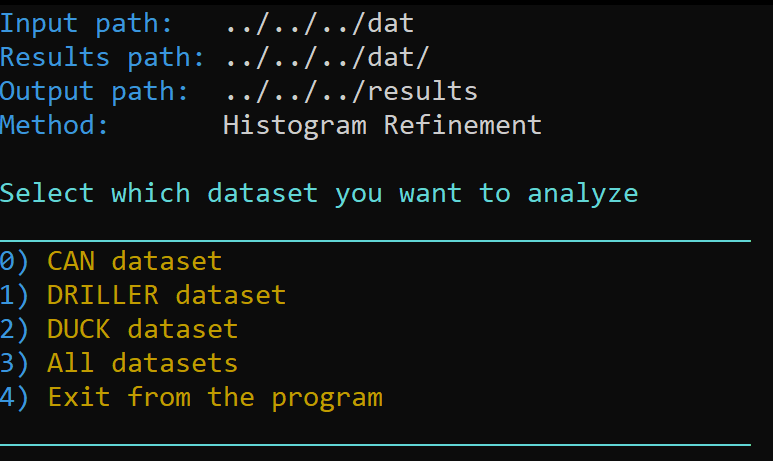
\includegraphics[width=.5\linewidth]{Images/menu.png}
\caption{Appearance of the initial Menu.}
\label{menu}
\end{figure}

\begin{figure}[H]
\begin{subfigure}{.5\textwidth}
  \centering
  % include second image
  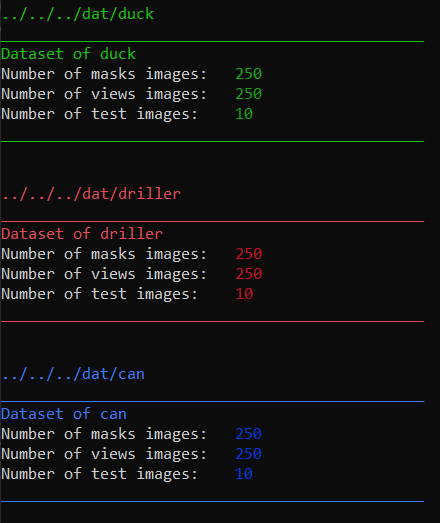
\includegraphics[width=.9\linewidth]{Images/parallel_init.png}
\caption{Initial program log with the description of the input.}
\end{subfigure}
\begin{subfigure}{.5\textwidth}
  \centering
  % include second image
  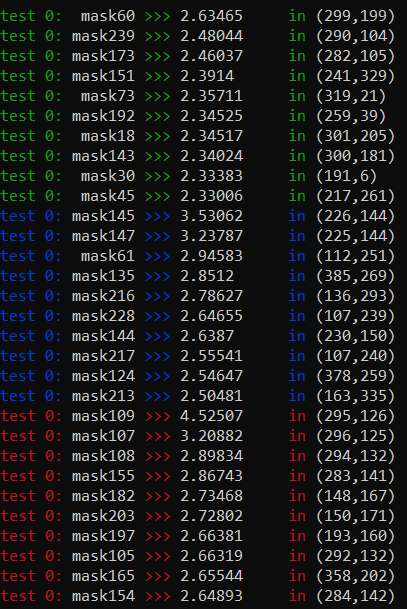
\includegraphics[width=.9\linewidth]{Images/parallel_run.png}
\caption{Log with image number, matched mask, score and position of the mask.}
\end{subfigure}
  \caption{Logs during execution on all datasets in parallel.}
  \label{parallel_log}
\end{figure}
\subsection{Code Organisation}
The program is composed by 13 files organized, looking to their functionalities, into the following sets:
\begin{itemize}
\item{\textbf{Template matching}\\
It's composed by the \texttt{TemplateMatching.hpp} and \texttt{TemplateMatching.cpp} files that implement the class used to perform the two methods for estimating the best matches.
}
\item{\textbf{$\gamma$-transform}\\
It's composed by the \texttt{GammaTransform.hpp} and \texttt{GammaTransform.cpp} files that implement the class used to perform the $\gamma$-transform. 
}
\item{\textbf{Menu}\\
It's composed by the \texttt{Menu.hpp} and \texttt{Menu.cpp} files that implement the static class with parser of the command line arguments and management of menu printing on screen.
}
\item{\textbf{Main activity}\\
It's composed by the \texttt{Project.hpp} and \texttt{Project.cpp} files that implement the main function and manage threads to perform Template Matching.
}
\item{\textbf{Canny detection}\\
It's composed by the \texttt{CannyDetector.hpp} and \texttt{CannyDetector.cpp} files that implement the class used to perform Canny Detection on a specific image.
}
\item{\textbf{Storing of best matches}\\
It's composed by the \texttt{BestResults.hpp} and \texttt{BestResults.cpp} files that implement the classes:
\begin{itemize}
\item{\texttt{Result}\\
it defines the main information to be stored for each result of the matching approaches and implements the methods needed to access these fields.
}
\item{\texttt{BestResults}\\
it constructs the buffer of results and manages its update.
}
\end{itemize}
}
\item{\textbf{Utility constants}\\
It's composed by the \texttt{Utility.hpp} file and declares some useful variables:
\begin{itemize}
\item{Colours used in log printing}
\item{Colours used in Menu}
\item{Colours used for printing the mask name and the edges of the matched mask in the result image}
\item{Gamma values for Gamma Transform}
\item{Threshold values for Canny Detection}
\item{Name of sub-folders needed to load images of datasets provided by the user}
\end{itemize}
}
\end{itemize}
\end{document}